\chapter{Modelling colorectal cancer methylation data with \texttt{methdemon}}
\label{chapter:methylation}


\section{Introduction}
The main motivation for the development of \texttt{methdemon} is to infer
evolutionary properties of colorectal cancer (CRC) from methylation data. CRC
is the third most common cancer worldwide, with over $40000$ new cases
diagnosed in the UK each year on average \cite{noauthor_bowel_2015}. The scale
of this issue is not the only motivating factor, as insights into the
evolutionary dynamics of colorectal cancer could lead to the better
understanding of how other adenocarcinomas progress. CRC is characterised by the
accumulation of genetic and epigenetic mutations in colonic cells
\cite{fleming_colorectal_2012}. The most common type of CRC is adenocarcinoma,
which arises from the epithelial cells lining the colon, covering the majority
of cases. The tumour forms hierarchical cell structures similar to those of
normal tissue, organising into crypt-like glands
\cite{ponz_de_leon_pathology_2001}. The tumour spreads by the process of gland
fission \cite{preston_bottom-up_nodate}, which is similar to the branching
processes seen in normal crypts \cite{almet_multicellular_2018}. \par
In this chapter, I will use the inference workflow introduced in chapter
\ref{chapter:methdemon} to infer evolutionary properties of colorectal cancer
from methylation data. My approach, similar to that of
\cite{gabbutt_fluctuating_2022, gabbutt_evolutionary_2023}, is not the first
investigation of whether methylation arrays can uncover evolutionary properties
of colorectal cancer, as there have been efforts to infer strength of selection
\cite{siegmund_high_2011} and the evolutionary history \cite{hong_using_2010} of
the primary tumour. The model presented in chapter \ref{chapter:methdemon} is
informed by the assumptions used in these works, as well as other recent models
of colorectal cancer evolution and progression.

\section{Data collection}
The data used in this study were provided by Dr Darryl Shibata from the Keck
School of Medicine at the University of Southern California. The data consist
of DNA methylation arrays sequenced from multiple glands within colorectal
tumours post-surgery. All samples are anonymised. The arrays were obtained from
bulk samples of tumour glands, which means that the data are nominally not
single-cell resolved. Each tumour sample consists of $8$ glands, with each
gland's array containing some $850000$ CpG sites. The arrays were obtained
using the Illumina Infinium MethylationEPIC BeadChip array. The data were
pre-processed by Dr Shibata to remove low-quality samples and normalise the
arrays. The sample purity was high, with the vast majority of cells in the
samples being tumour cells.

\section{Results}
\subsection{Identification of fCpG loci in colorectal cancer}
The first step in the analysis was to identify the fCpG loci in the data. As
multiple samples come from the same tumour, a larger cohort of samples is
needed to reliably identify fCpG loci using the methods described by
\cite{gabbutt_evolutionary_2023}, i.e. isolating a set of CpG loci which are
the least informative about the methylation state across the cohort. Dr Gabbutt
ran the analysis on colorectal cancer data from the Cancer Genome Atlas (TCGA)
and identified $1258$ fCpG loci. For comparison, I ran a similar analysis only
on the data provided by Dr Shibata and identified a set of some $950$ loci. Of
these, only $120$ were common to both sets. The discrepancy is likely due to
the small sample size of the data provided by Dr Shibata. The fCpG loci
identified in one of the samples are shown in figure \ref{fig:fCpG_loci_S},
with additional figures in appendix \ref{app:inference}.

\begin{figure}[h]
    \centering
    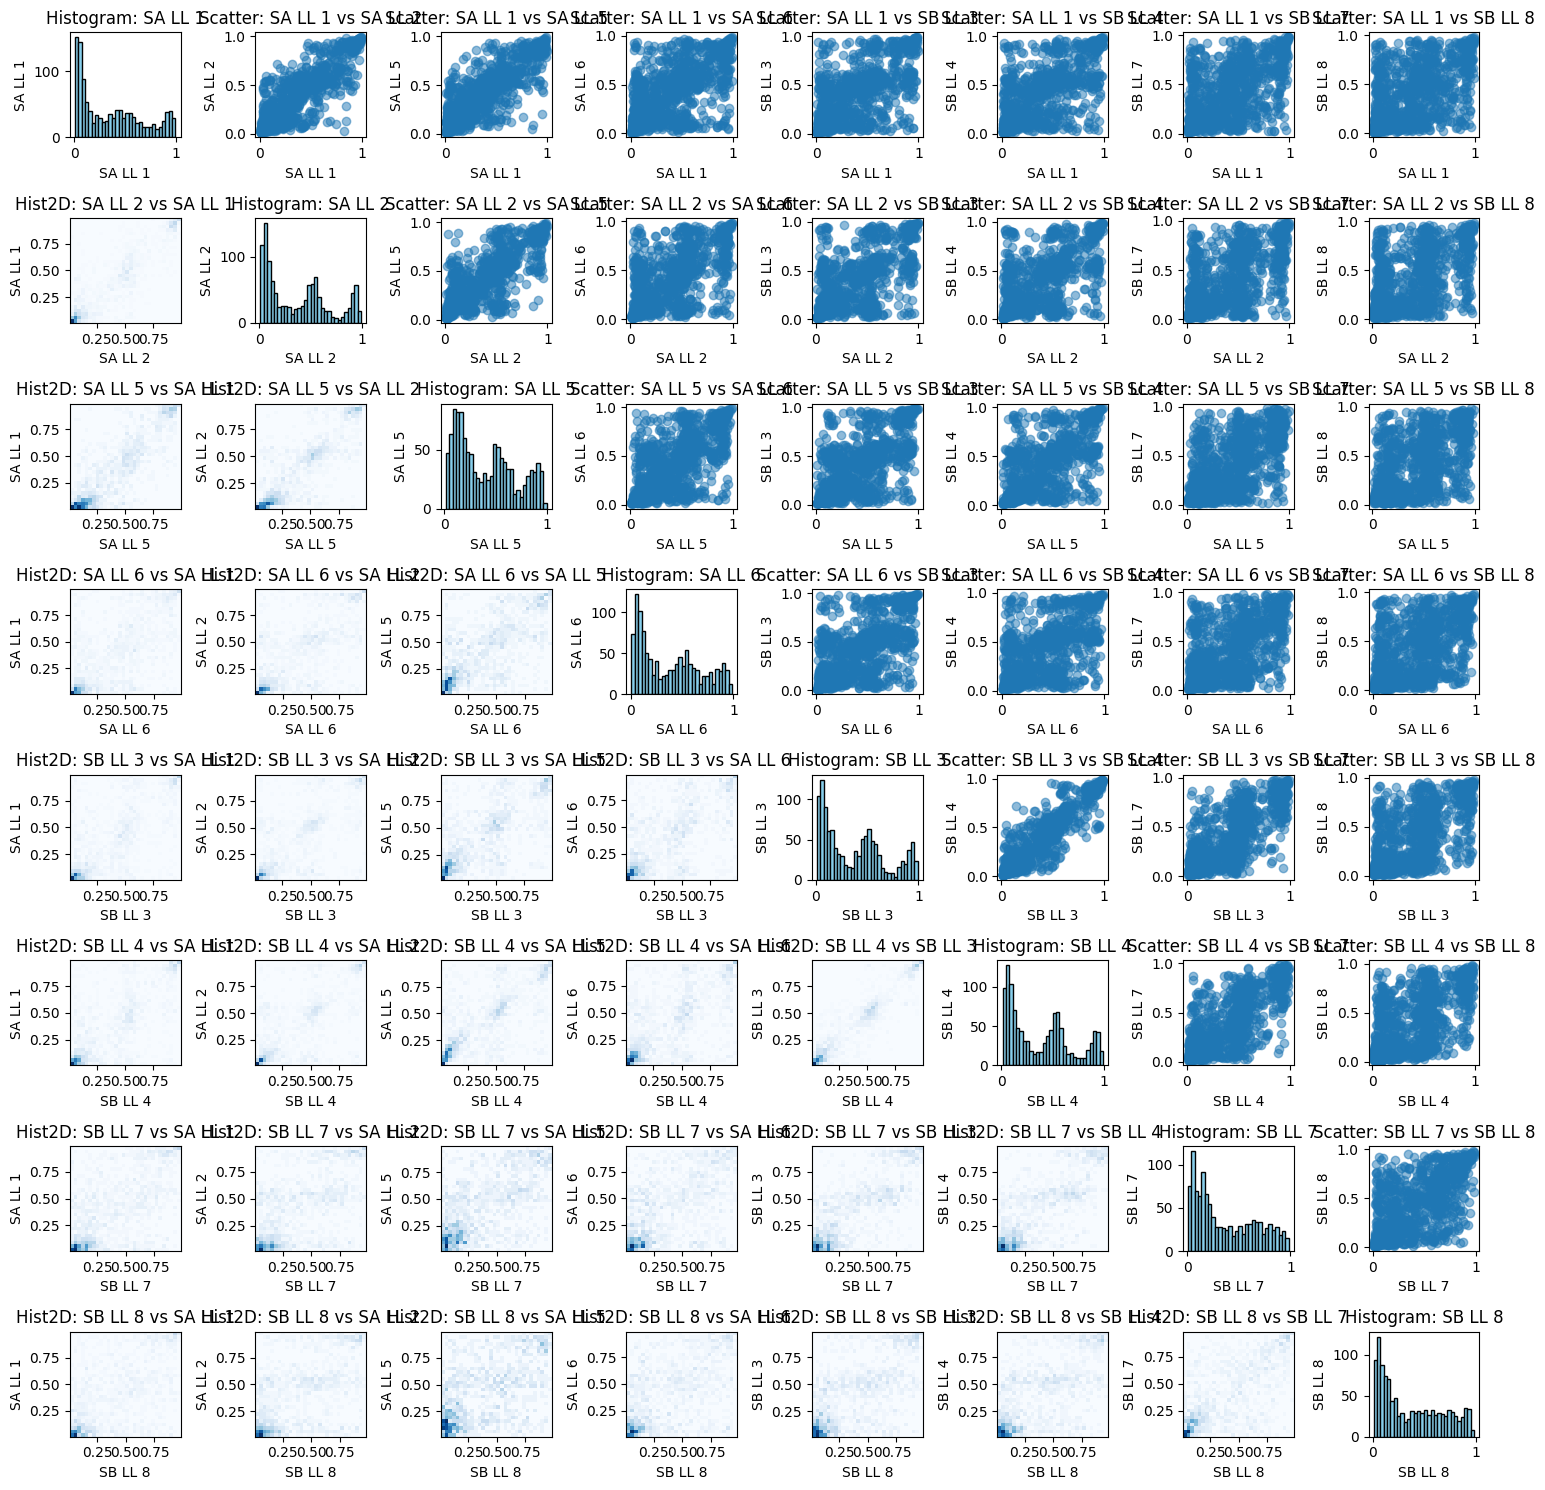
\includegraphics[width=\textwidth]{Chapter_5/figures/fCpG_loci_S.png}
    \caption{Visualisation of the set of fCpGs for tumour samples from patient
    S. \textbf{diagonal} --- histograms of fCpG arrays for each gland;
    \textbf{above diagonal} --- scatter plots of correlations between glands;
    \textbf{below diagonal} --- $2$D histograms of the above-diagonal plots,
    showing the density of points.}
    \label{fig:fCpG_loci_S}
\end{figure}


\subsection{Spatial proximity predicts similarity between fCpG arrays}
With the assumed hierarchical structure of the tumour in mind, it should make
sense intuitively that glands which are spatially close to each other likely
diverged more recently than glands which are further apart. As a result, they
have spent less time evolving independently and should have more similar fCpG
arrays. To test this hypothesis, I calculated the inter-gland distance matrix
for each tumour sample. The resulting matrices show a clear correlation between
side and distance values. The distance matrix for one of the samples is shown
in figure \ref{fig:gland_dist_S} for tumour S, and in appendix
\ref{app:inference} for the other samples.

\begin{figure}[h]
    \centering
    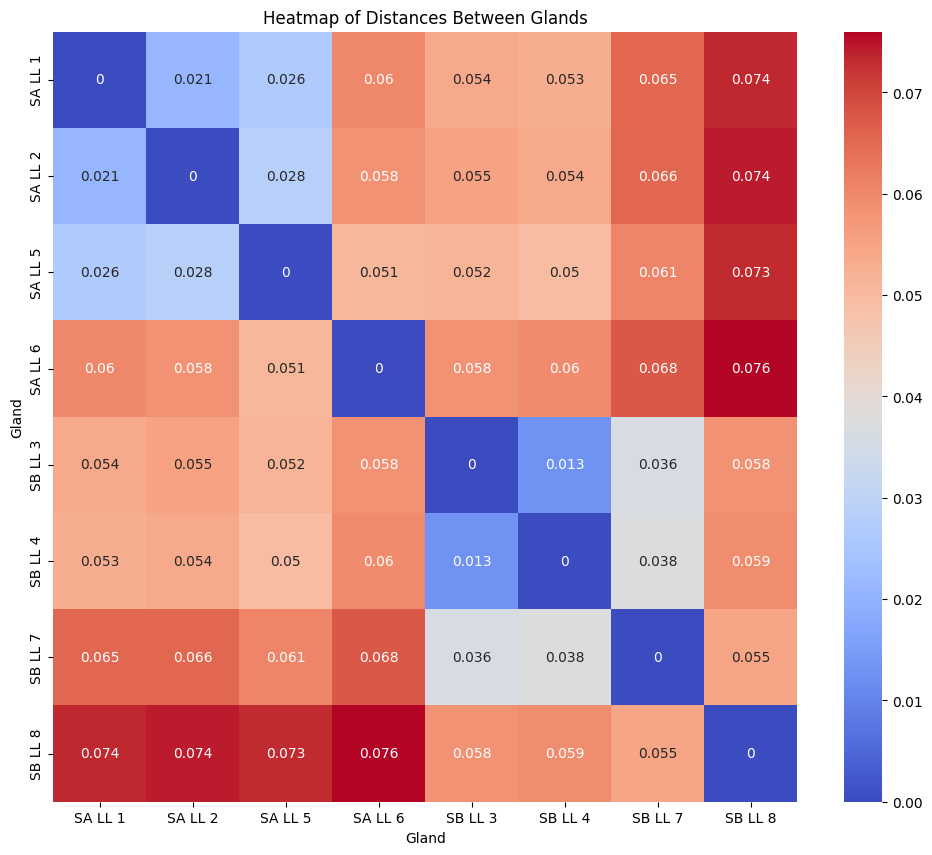
\includegraphics[width=\textwidth]{Chapter_5/figures/gland_dist_S.png}
    \caption{The inter-gland distance matrix for tumour S. The distance values
    are, broadly speaking, higher between distant glands than ones from the same
    side of the tumour (A or B).}
    \label{fig:gland_dist_S}
\end{figure}

\subsection{Development of the \texttt{methdemon} model}
The \texttt{methdemon} model was developed for the purpose of simulating the
data provided by Dr Shibata. The model's assumptions are based on the general
understanding of colorectal cancer evolution and, translated into the language
of an agent-based model, are as follows:

\begin{enumerate}[(i)]
    \item \textbf{A single cell forms the first gland and initiates tumour
        growth.} This assumption skips over the process of tumorigenesis,
        during which a cell accumulates mutations and becomes malignant
        \cite{tariq_colorectal_2016}. This is a simplification to be sure, but
        a reasonable one, given that the focus of this work is on the
        evolutionary dynamics of the tumour rather than its initiation.
    \item \textbf{The rate of driver mutations is Poisson distributed and
        identical for all cells.} This assumption is consistent with most
        models of tumour evolution \cite{metzcar_review_2019,
        niida_modeling_2021}.
    \item \textbf{The cell population within a gland grows exponentially and is
        well-mixed.} While not necessarily consistent with the biology of a
        solid tumour, this assumption allows for more efficiency in the
        simulation as opposed to a multi-level spatial model. Further, as the
        data discussed in chapter \ref{chapter:methylation} is obtained from
        bulk samples of tumour glands, this assumption is not unreasonable.
        \label{item:well_mixed}
    \item \textbf{Once a gland reaches a certain size, which we call the
        carrying capacity, the population undergoes steady-state turnover
        according to the Moran process.}
    \item \textbf{At carrying capacity, a gland has a certain probability of
        undergoing fission, which splits the gland's population randomly into
        two.} As a consequence of assumption (\ref{item:well_mixed}), fissions
        do not take into account a gland's spatial organisation.
    \item \textbf{Gland fission occurs as a neutral spatial branching process.}
        The previous two assumptions and this one together form the basis of
        the model's spatial dynamics. While there are other mechanisms of
        colorectal adenocarcinoma progression, gland fission is the principal
        way in which the tumour grows \cite{preston_bottom-up_nodate}. The
        assumption of neutrality in the spatial branching process is consistent
        with the findings of \cite{sottoriva_big_2015}. Additionally, this
        assumption is based on the fact that the data used in this study only
        contains information about whether a gland was sample from side A or B,
        without any further spatial information other than the approximate size
        of the full tumour.
\end{enumerate}

\subsection{Higher deme carrying capacity requires stronger selection to
recapitulate the data}
To begin the analysis of cancer data using the \texttt{methdemon} model, I tested the
ranges of parameters based on the assumption that each cancer cell has infinite
proliferative potential. This would mean setting the carrying capacity of a gland
to about $10000$ cells, which is consistent with the size of the glands in the
literature \cite{sottoriva_big_2015} and our data. Due to the glandular
structure of the tumour, this is an effectively neutral model, as selection
acts within glands but not between them, leading to progressive diversification
of the population, as discussed in chapter \ref{chapter:trajectories} and
\cite{noble_spatial_2022}.\par

\begin{figure}[h]
    \centering
    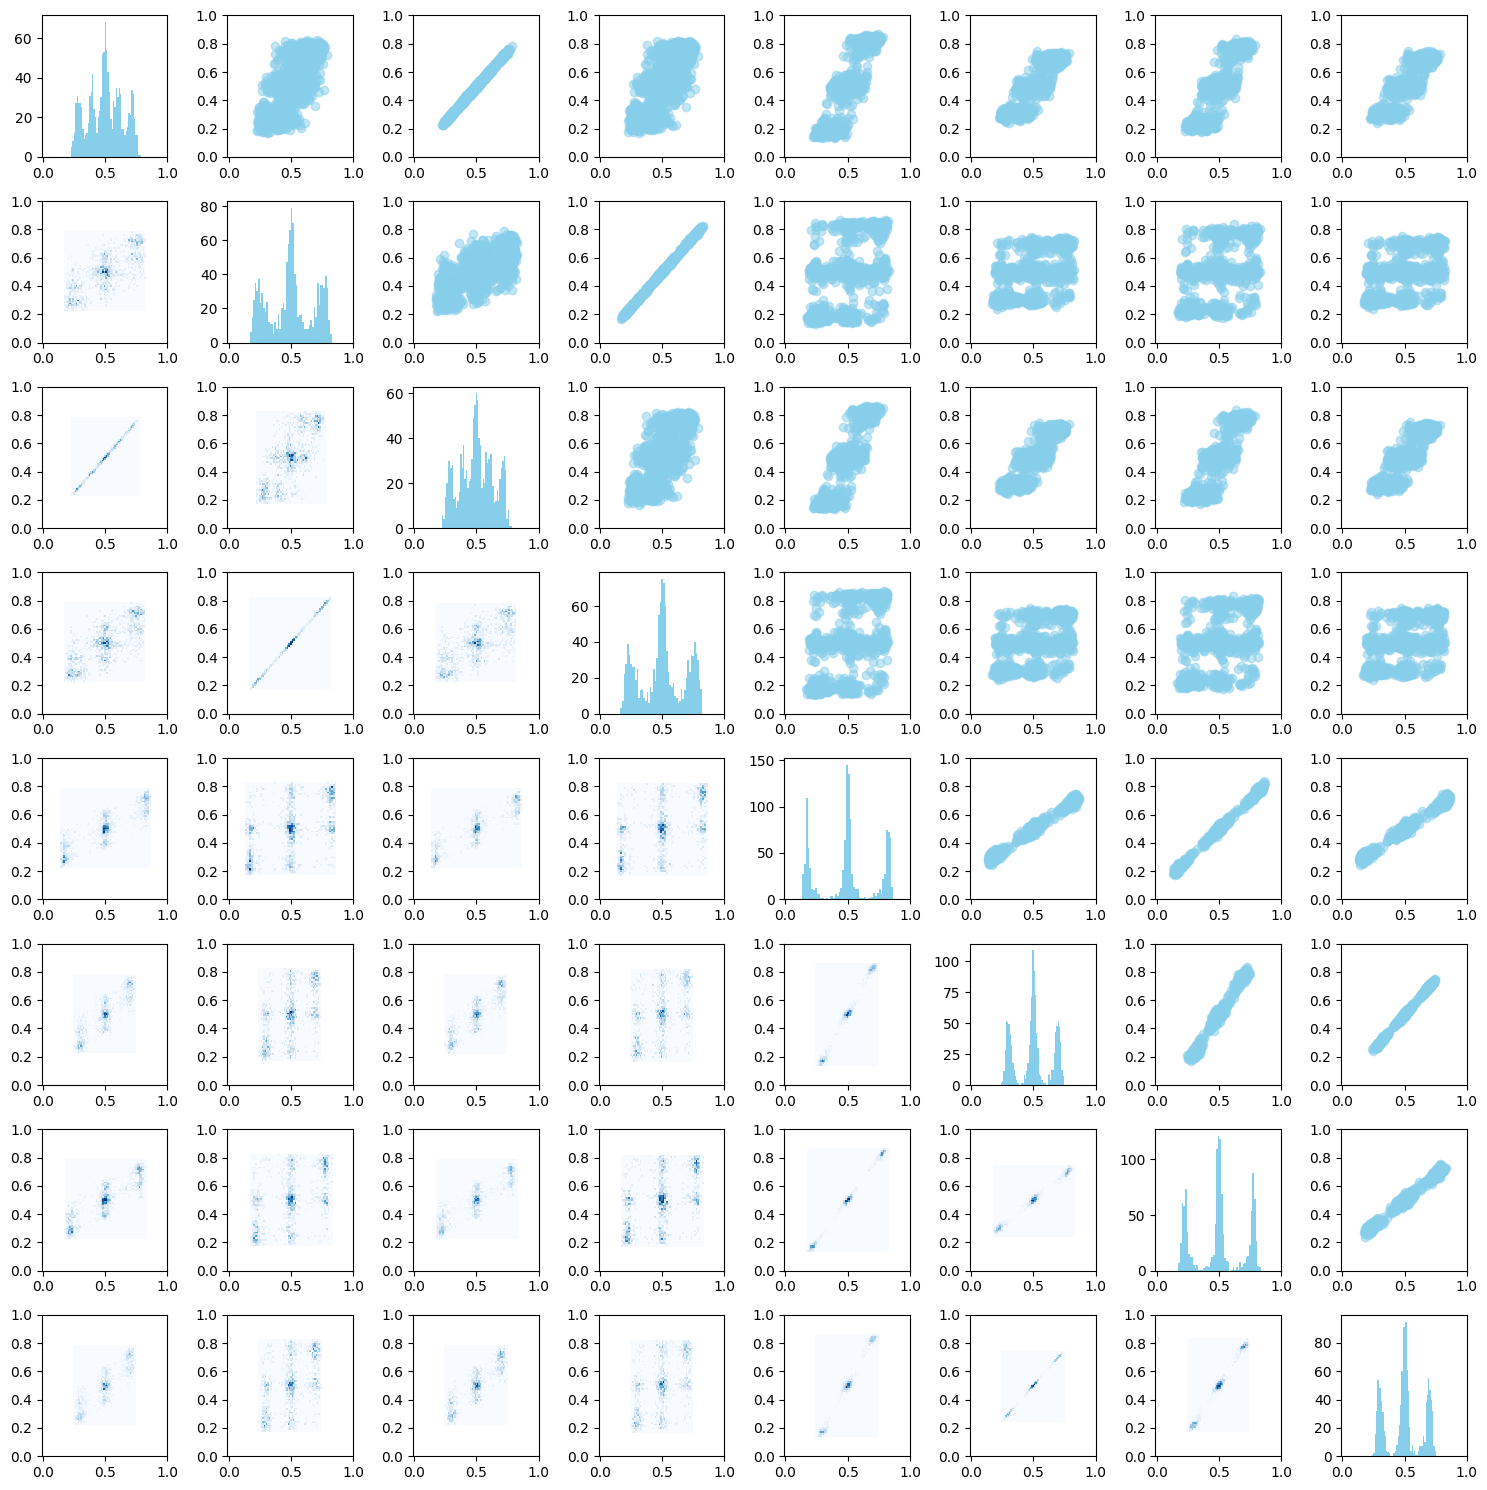
\includegraphics[width=\textwidth]{Chapter_5/figures/10000plot.png}
    \caption{Visualisation of the output fCpG arrays from the
    \texttt{methdemon} model with weak selection ($s=0.1$) and deme carrying
    capacity $10000$. While The individual gland distributions are trimodal and
    the inter-gland correlation plots show epigenetic switching between sides,
    the distributions have narrowed down towards the mean ($0.5$) considerably.
    This happens in the case when the epimutation rate outpaces the tumour
    growth rate.}
    \label{fig:methdemon_weak_selection}
\end{figure}

\begin{figure}[h]
    \centering
    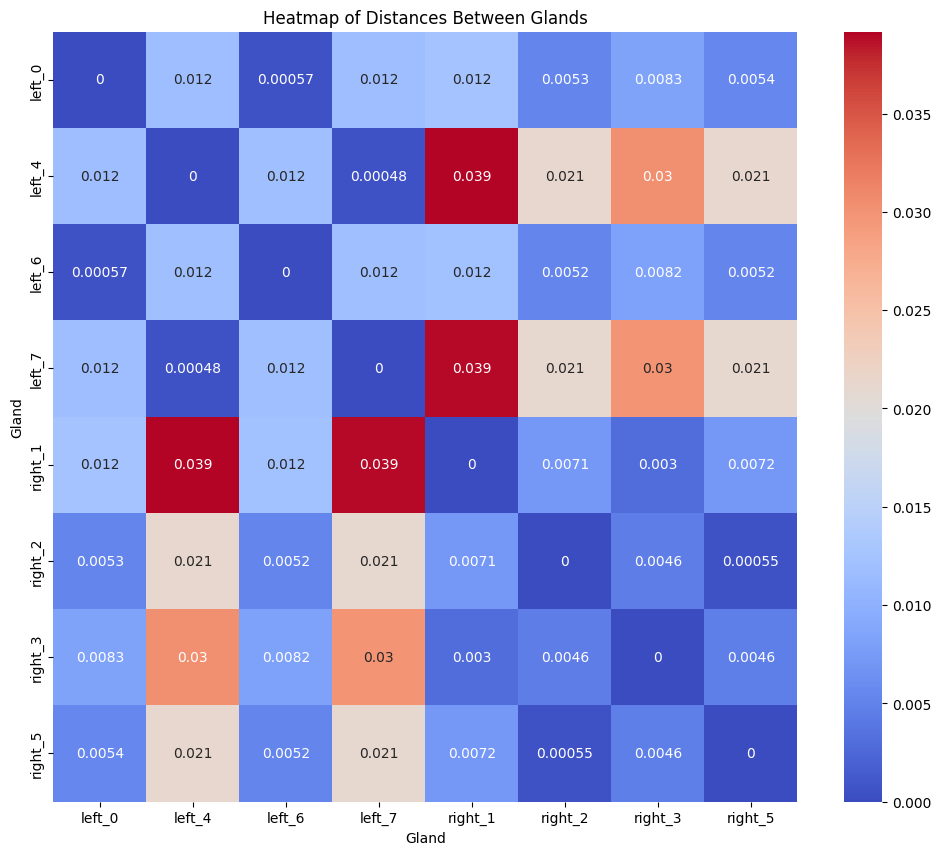
\includegraphics[width=\textwidth]{Chapter_5/figures/10000dist.png}
    \caption{Inter-gland distance matrix for the output fCpG arrays from the
    \texttt{methdemon} model with weak selection ($s=0.1$). While the distance
    values between glands on opposite sides of the tumour are still on average
    higher than within one side, the numerical values are around an order of
    magnitude off those observed in data.}
    \label{fig:methdemon_weak_dist}
\end{figure}

As a first test, I ran the model with weak selection, $s=0.1$. The resulting
outputs are shown in figures \ref{fig:methdemon_weak_selection} and
\ref{fig:methdemon_weak_dist}. There are a few notable features about the
output fCpG arrays and the distance matrix. The most obvious is that the peaks
associated with homozygous methylation and demethylation states have moved
towards the middle. This is to be expected, as we are treating all $10000$ cells
in a deme as being able to divide ad infinitum, leading to a lot of stochastic
noise. This is a consequence of the time spent in turnover, and is adjusted by
increasing the fission rate. However, the distance matrix shows that the glands
are still very similar to each other, especially when compared to the data. This
is likely due to the fact that there is only a small probability of a partial or
full sweep of a lineage within a gland. The similarity is a consequence of the
large deme carrying capacity, which allows for a lot of stochastic noise to
accumulate over time but lowers the probability of fixation in the weak
selection regime. Increasing the selection coefficient to $s=0.3$ leads to more
divergence between the glands, since emerging lineages are more likely to fully
or partially sweep the gland's population and establish more distinct fCpG
arrays between glands. However, as discussed in chapter \ref{chapter:methdemon},
strong selection can quickly become problematic in an ABM like this due to the
accumulation of advantageous drivers. An example of strong selection at deme
size $10000$ is in appendix \ref{app:inference}. \par
Considering that the number of stem cells in a normal crypt is on the order of
$10$ \cite{gehart_tales_2019, gabbutt_fluctuating_2022}, with the total number
of cells in a crypt being on the order of $1000$, I next tested the model with
a deme carrying capacity of $100$ i.e. about $1\%$ of the total cell population
in the gland. The currently available data supports this percentage as a
reasonable estimate of the proportion of cancer stem cells (CSCs) in colorectal
cancer \cite{obrien_human_2007, munro_cancer_2018}. In this case, the model's
outputs are as expected, with the fCpG arrays diverging over time even with no
or weak selection. Examples are shown in figures
\ref{fig:methdemon_weak_selection_small} and
\ref{fig:methdemon_weak_dist_small}.

\begin{figure}[h]
    \centering
    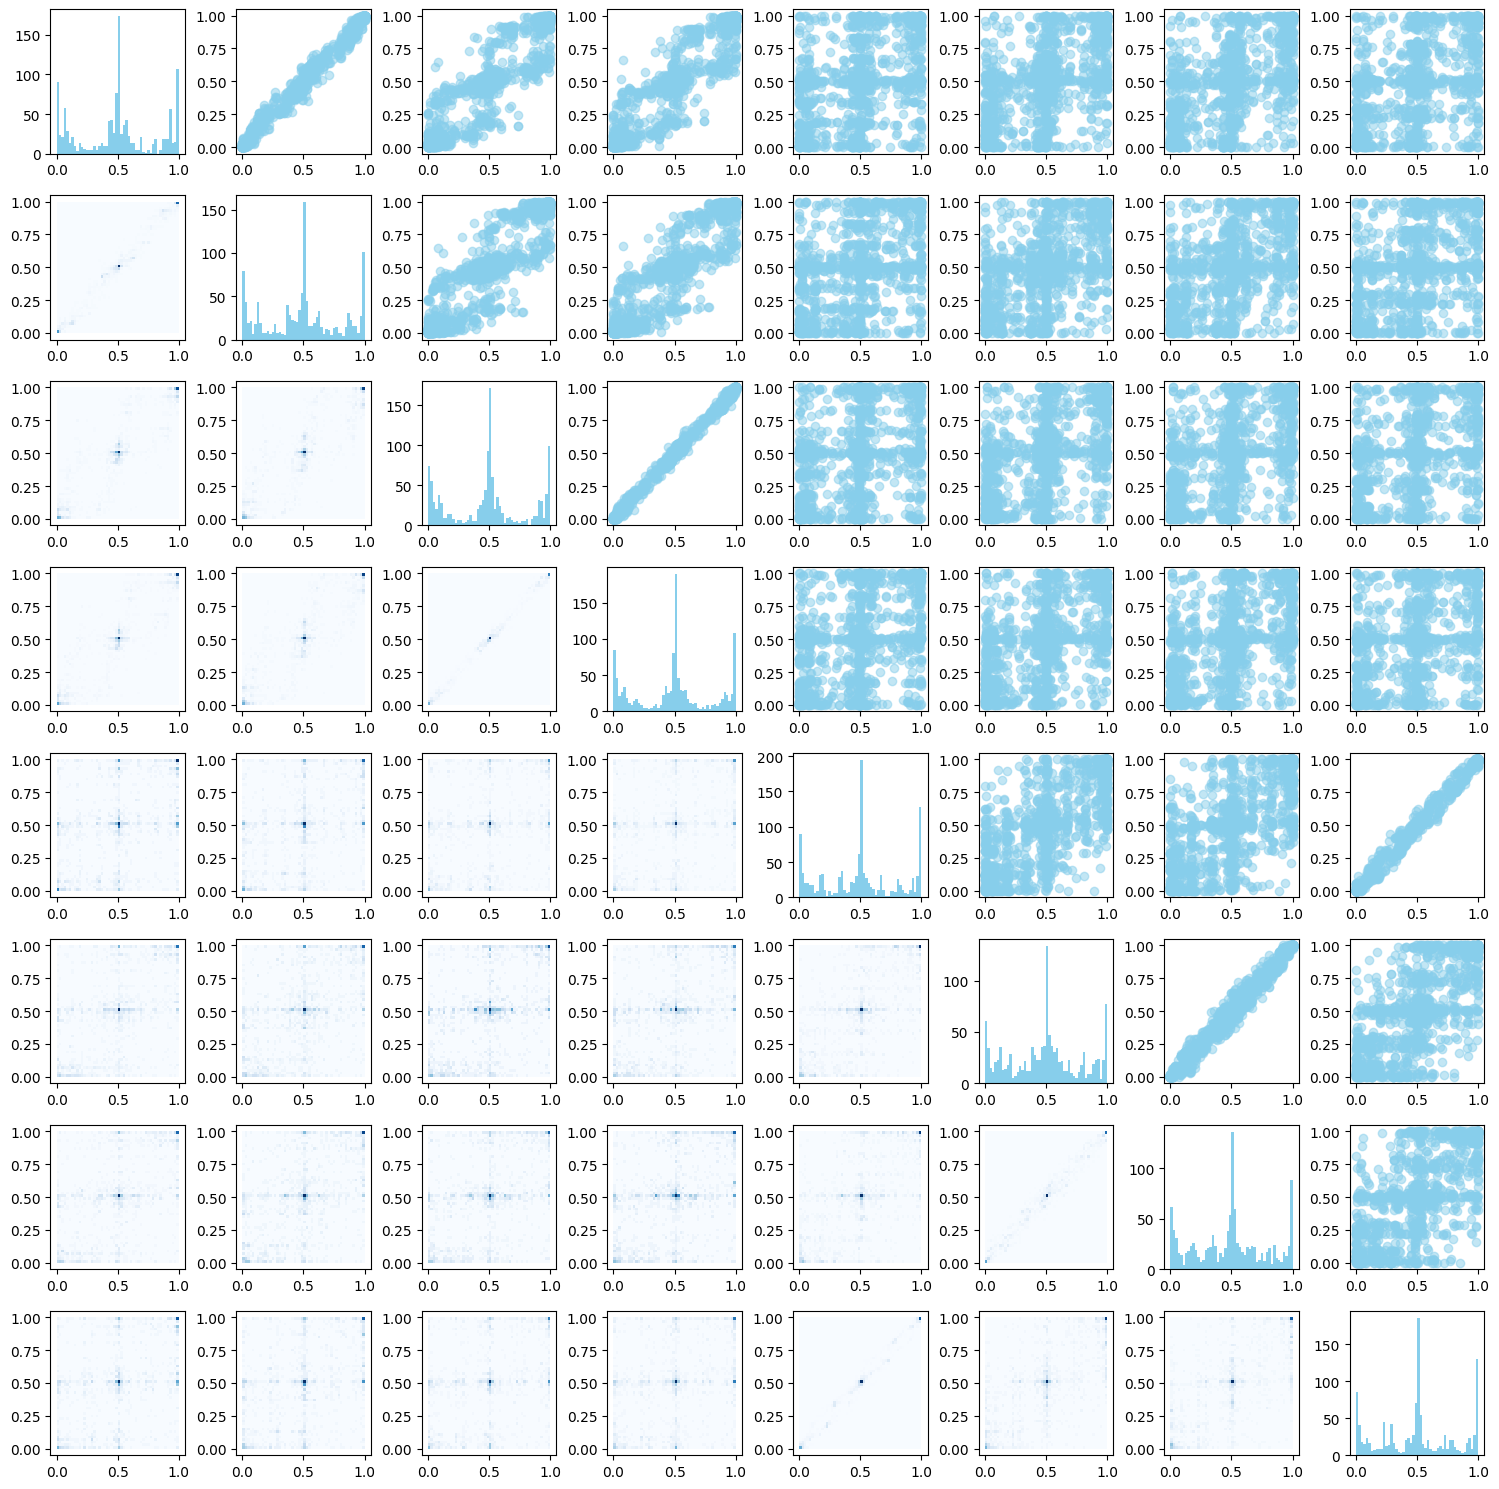
\includegraphics[width=\textwidth]{Chapter_5/figures/100plot.png}
    \caption{Output fCpG arrays from the \texttt{methdemon} model with weak
    selection ($s=0.1$) and deme carrying capacity $100$. The outputs of runs
    with a lower deme carrying capacity reflect the data better than larger
    deme carrying capacity.}
    \label{fig:methdemon_weak_selection_small}
\end{figure}

\begin{figure}[h]
    \centering
    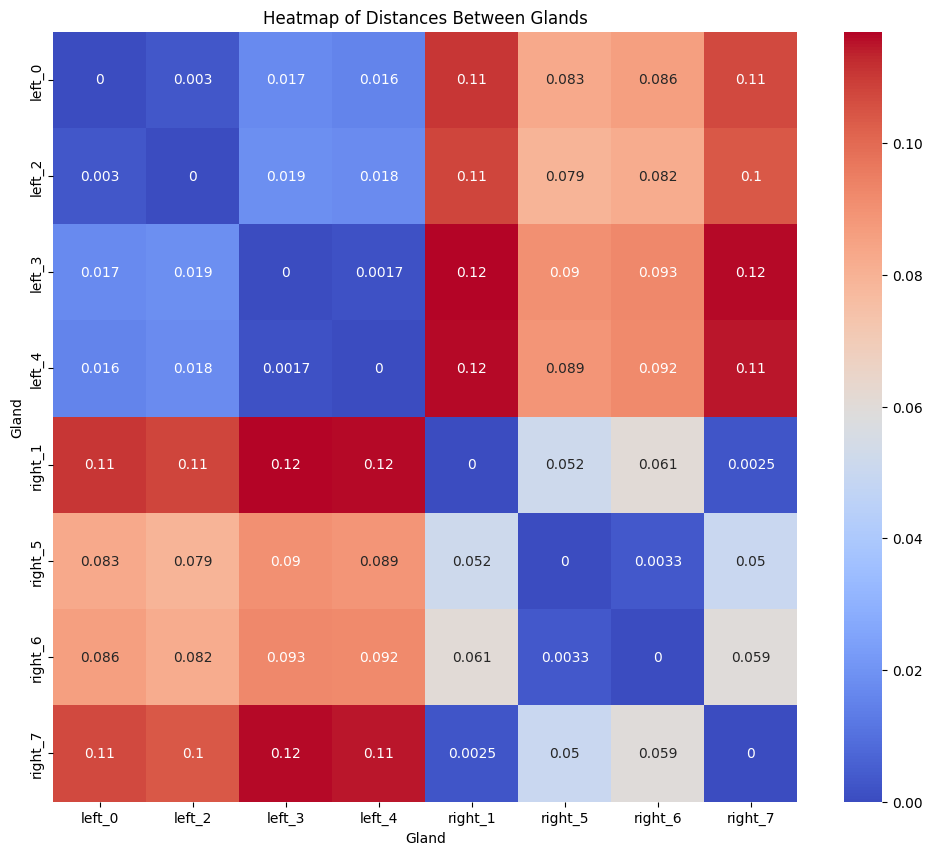
\includegraphics[width=\textwidth]{Chapter_5/figures/100dist.png}
    \caption{Inter-gland distance matrix corresponding to the run from figure
    \ref{fig:methdemon_weak_selection_small}. The values in the distance matrix
    are comparable to those seen in the molecular data sets.}
    \label{fig:methdemon_weak_dist_small}
\end{figure}
\clearpage

\subsection{Parameter inference from colorectal cancer data}
\subsubsection{Regular model}
Having established \texttt{methdemon}'s ability to output data which resembles
observations, I next attempted to fit the model to the colorectal cancer data.
For this, I used the ABC workflow described in chapter \ref{chapter:methdemon}.
Considering the results of the previous section, I set the deme carrying
capacity to $100$ for all inference runs. I made this choice as there is no
evidence to suggest different numbers of stem cells across tumours or even
glands within a tumour. Furthermore, having the deme carrying capacity as a free
parameter would slow down the inference process significantly.
In the first instance, I ran the inference with parameter ranges given in table
\ref{tab:inf_ranges}. The results of the inference are shown in figure
\ref{fig:inference_1}, with more details in appendix \ref{app:inference}.

\begin{table}[ht]
\centering
\begin{tabular}{|l|l|l|}
\hline
Parameter & Prior \\
\hline
methylation rate & $U(0, 0.1)$ \\
demethylation rate & $U(0, 0.1)$ \\
fission rate & $U(10^{-4}, 10^{-2})$ \\
driver mutation rate & $U(0, 10^{-2})$ \\
selective advantage & $U(0, 0.2)$ \\
\hline
\end{tabular}
\caption{Parameter priors for the first inference run.}
\label{tab:inf_ranges}
\end{table}

The first inference run did produce some results, but the posterior
distributions of some parameters remained broad. There are a few possible
reasons for this. Firstly, I intentianally used overly broad priors to see how
well the ABC workflow would delineate the parameter space. This choice makes the
inference process more dificult, as the prior distributions are not informative
and the parameter space is large. However, it allows for future runs with more
informative priors. The second reason may just be that the model is not able to
recover all of the parameters in its current form. Selective advantage and
driver mutation rate in particular seem to be difficult to infer for the model.
This could be due to the signature of selection being too weak in the model or
data (or both). It could also be down to the distance functions in the ABC
rejection step not being able to capture the differences between the arrays
well enough. Either way, the results prompted further testing with the important
change of log-transforming the parameters. This change allows for more efficient
exploration of the parameter space, as parameters are sampled on the same scale
and steps between generations will cover more of the space.

\begin{figure}[h]
    \centering
    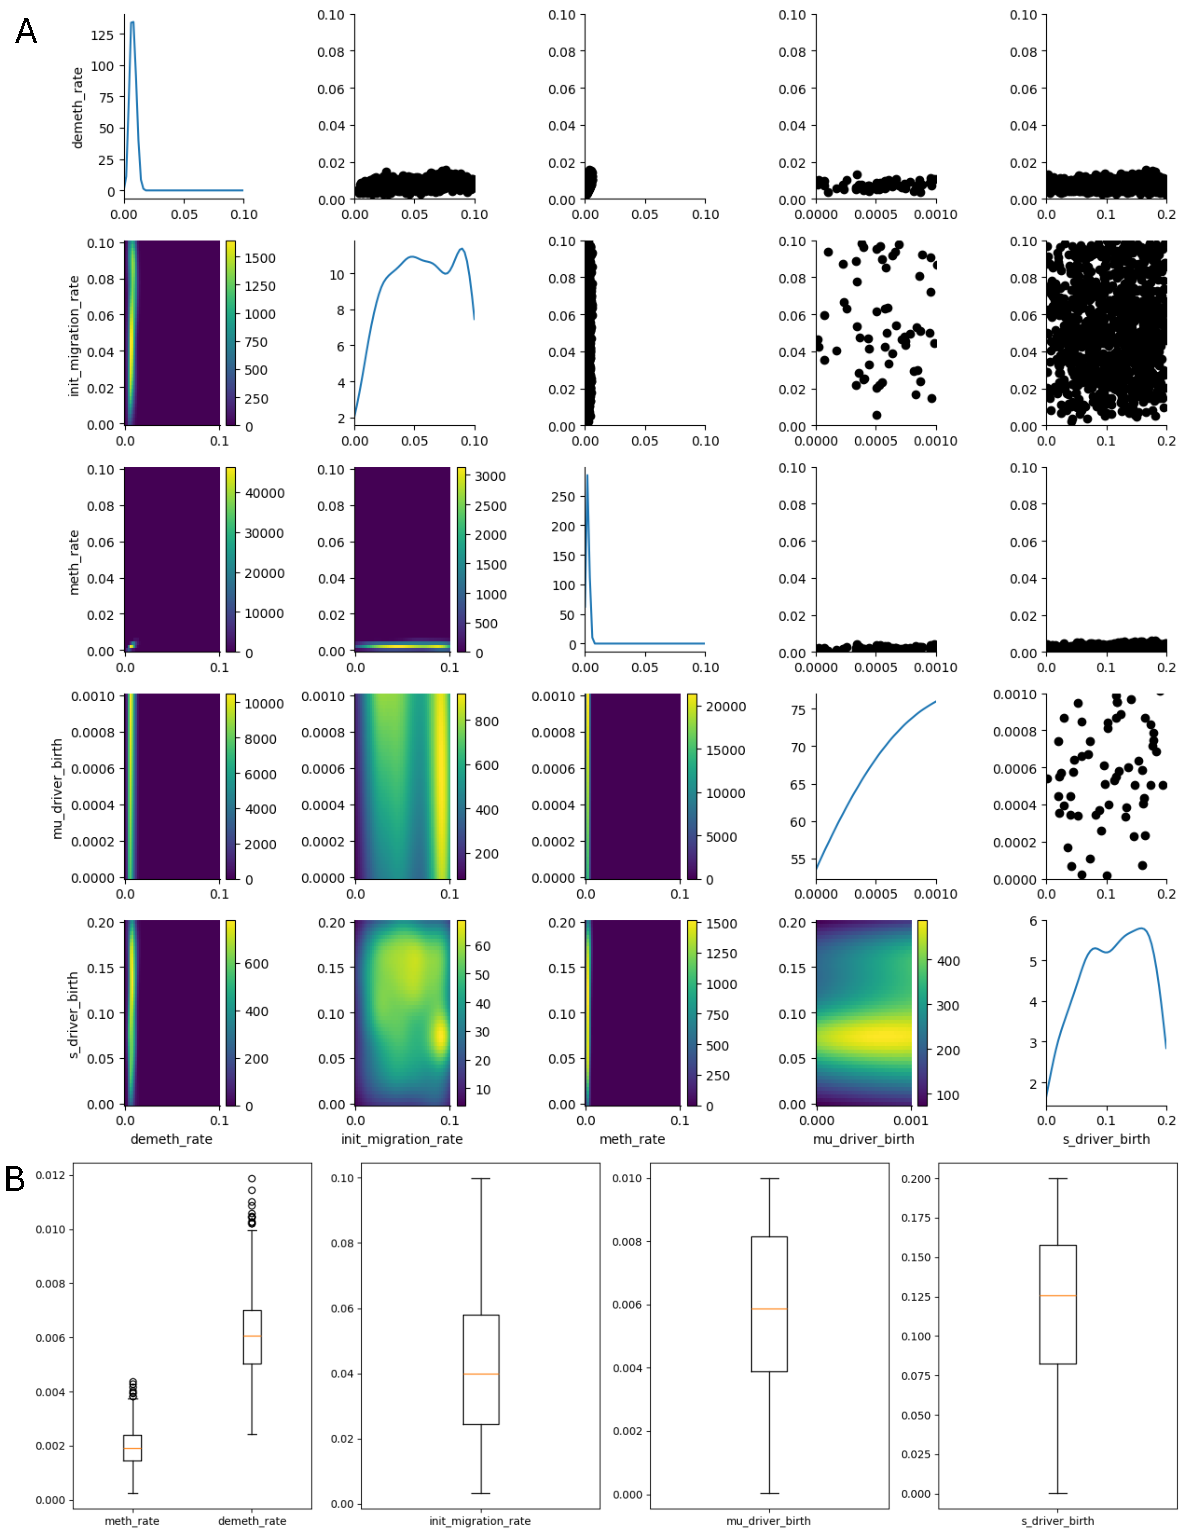
\includegraphics[width=\textwidth]{Chapter_5/figures/inference_raw/inference_1.pdf}
    \caption{Inference outputs from the first run, performed by sampling
    parameters from uniform priors on the original scale. While the epimutation
    rates' posteriors narrow down considerably, other parameter distributions
    remain broad - likely due to too coarse traversal of the parameter space.
    \textbf{A} --- posterior distributions of fCpG fluctuation rates have
    narrowed down rapidly, but other parameters' posteriors remain broad.
    \textbf{B} --- box plots of the posteriors show that the model is not able
    to resolve the effects of selection from the data, and leaves a lot of
    uncertainty in the fission rates.}
    \label{fig:inference_1}
\end{figure}
\clearpage

\subsubsection{Log-transformed model}
The second inference run was done with similar parameter ranges as the first.
The log-transformed parameter ranges are give in table \ref{tab:inf_ranges_log}
and the results of the inference are shown in figure \ref{fig:inference_2}, with
more details in appendix \ref{app:inference}. All log transformations were
done with base $10$.

\begin{table}[ht]
\centering
\begin{tabular}{|l|l|l|}
\hline
Parameter & Prior \\
\hline
log methylation rate & $U(-4, -2)$ \\
log demethylation rate & $U(-4, -2)$\\
log fission rate & $U(-3.3, -1)$\\
log driver mutation rate & $U(-5, -2)$\\
selective advantage & $U(0, 0.2)$\\
\hline
\end{tabular}
\caption{Log-transformed priors for the second inference run.}
\label{tab:inf_ranges_log}
\end{table}

The results of the second inference run are more promising than the first, with
the fission rate posterior distribution being considerably narrower. However,
selection and driver mutation rate are still difficult to narrow down. This
further supports the idea that the model is not able to detect weak selection
at the gland level.

\begin{figure}[h]
    \centering
    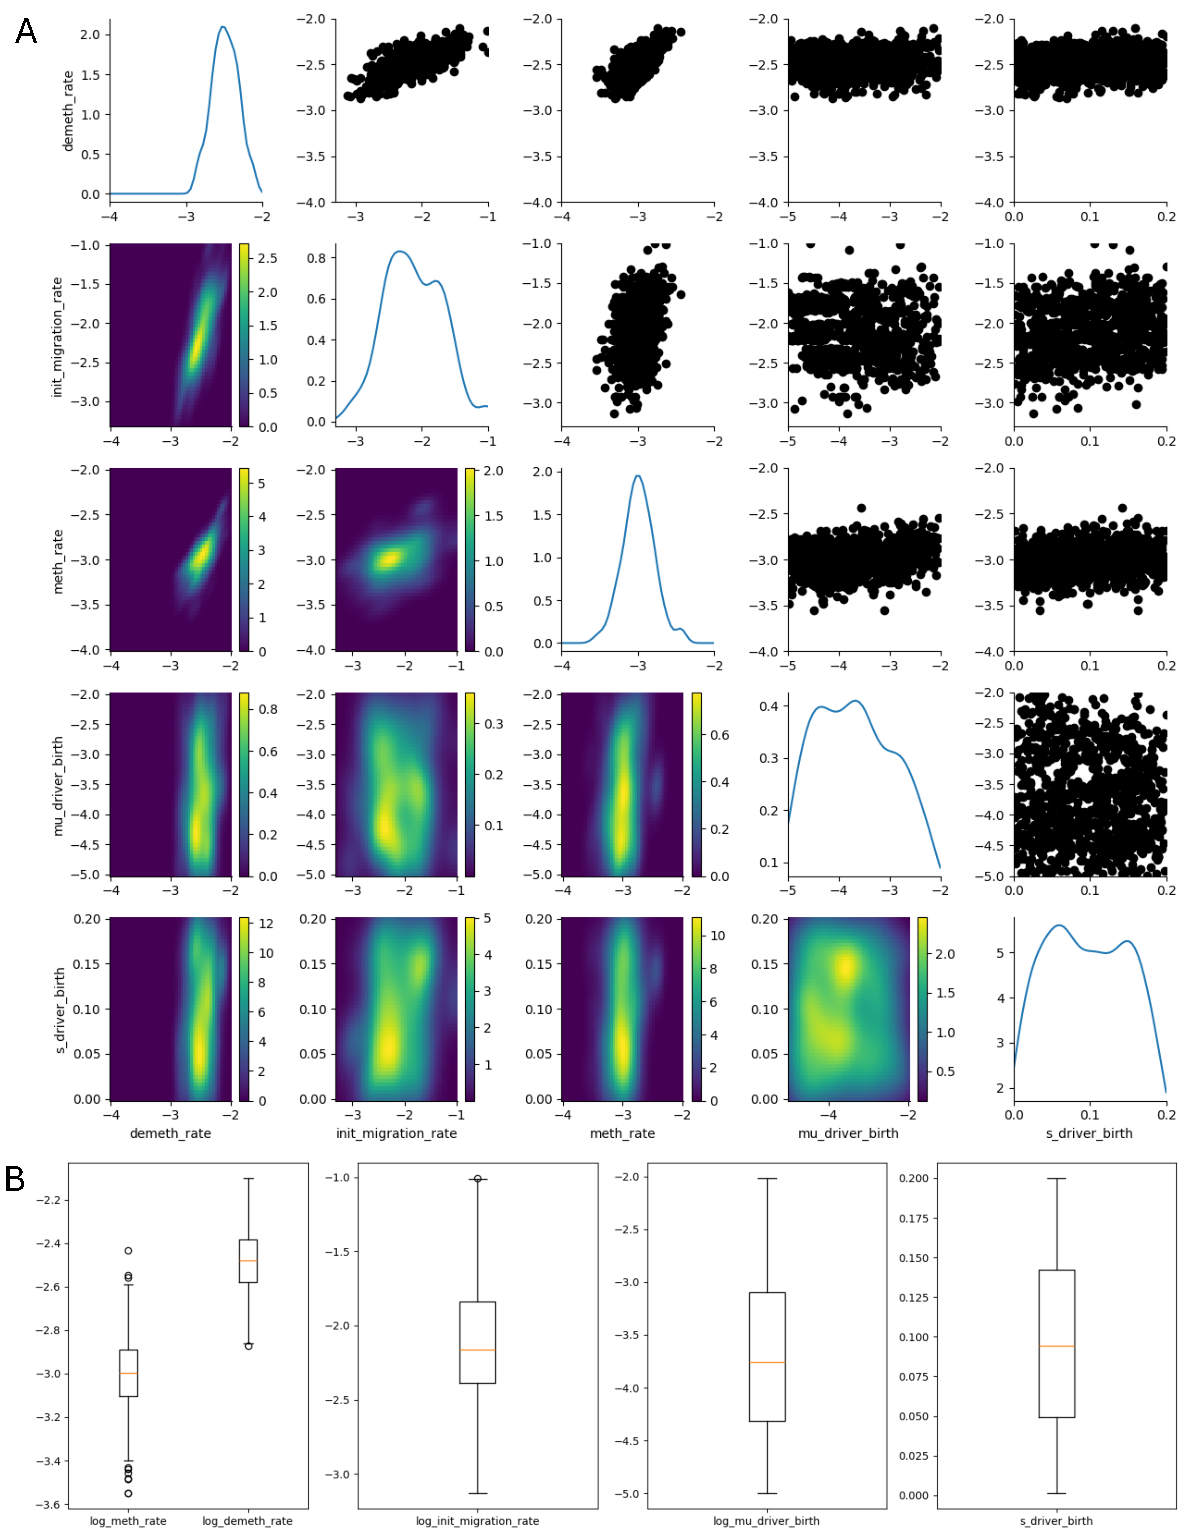
\includegraphics[width=\textwidth]{Chapter_5/figures/inference_raw/inference_S.pdf}
    \caption{Inference outputs from the alternative run, performed by sampling
    parameters from uniform priors on the log-transformed scale. The posterior
    distribution of deme fission has now narrowed down in a similar way to the
    epimutation rates, indicating a more efficient traversal of parameter space.
    \textbf{A} --- posterior distributions of fCpG fluctuation rates have
    narrowed similar to before, but now the fission rate's posterior is also
    narrower than before. Mutation rate and selective advantage are still not
    inferred by the model.
    \textbf{B} --- box plots of the posteriors.}
    \label{fig:inference_2}
\end{figure}
\clearpage

\subsection{Fast- and slow-growing tumours}
The data provided by Dr Shibata contains samples from different patients, with
each tumour being potentially at a different stage of growth. From exploratory
analysis, it seems that some tumours are growing faster than others, if we work
under the assumption that gland fission is the only mechanism of growth. This
hypothesis is supported by the inference results, as samples with higher values
in the inter-gland distance matrix tend to grow slower, and ones where gland
fCpG arrays are more similar have grown faster. The inferred median fission
rates are shown in table \ref{tab:fission_rates}. The inferred epimutation
rates are included in appendix \ref{app:inference}, in table
\ref{tab:inferred_epimutation_rates}.

\begin{table}[ht]
    \centering
    \begin{tabularx}{\textwidth}{|c|X|X|c|c|}
    \hline
    Tumour & Inferred median fission rate $[\text{cell}^{-1}\text{cell div}^{-1}]$ & $L_2$ half-norm & Tumour size [cm] & Stage \\
    \hline
    E & $0.0025$ & 0.481 & 6.1 & I \\
    \hline
    I & $0.017$ & 0.176 & 3.6 & III \\
    \hline
    J & $0.003444$ & 0.421 & 5 & III \\
    \hline
    S & $0.007$ & 0.295 & 6 & n/a \\
    \hline
    X & $0.0032$ & 0.338 & 2.5 & n/a \\
    \hline
    \end{tabularx}
    \caption{Inferred median fission rates for different tumours and their
    sizes. The $L_2$ half-norm of a tumour's inter-gland distance matrix appears
    to be inversely correlated with the inferred fission rate.}
    \label{tab:fission_rates}
\end{table}

As the inferred fission rates from table \ref{tab:fission_rates} are set per
cell per cell division, the fission rate per gland would be $100$ times higher,
or roughly in the interval $(0.1, 1)$ --- one order of magnitude less, or about
the same as the stem cell division rate. In my model, the tumour grows as a pure
birth branching process, meaning that the growth is exponential. Let $\phi$ be
the fission rate and $N(t)$ the number of glands in the tumour at time $t$. Then
\begin{equation}
    N(t) = e^{\phi t}N(0).
\end{equation}
As the tumour grows from a single gland, the time $\tau$ to reach a certain
size $N_\tau$ is
\begin{equation}
    \tau = \frac{1}{\phi}\log N_\tau.
\end{equation}
The literature does not provide clear estimates for cancer stem cell division
rates, but I think a reasonable estimate would be from about $1$ per month to
$1$ per week, or about $0.034$ to $0.1$ per day. This would mean that the time
to reach a size of $10^7$ glands would lie in the interval $(230, 7000)$ days,
or about $8$ months to $20$ years. This range is broad, and is not meant as a
precise estimate, but rather a sanity check of the model's outputs. Considering
that the orders of magnitude are correct, the model seems to be able to describe
the observed data well.

\section{Discussion}
In this chapter, I modelled colorectal cancer methylation data using
\texttt{methdemon} and the associated ABC workflow. A notable feature of the
data is that some samples show a clear bias towards either hyper- or
hypomethylation after filtering with the help of TCGA data. This was also the
case for fCpG arrays filtered using only the samples provided by Dr Shibata.
This suggests that the progenitor cell's methylation state is not necessarily
random, but could be affected by internal or external factors. Furthermore, I
developed the model under the assumption that methylation and demethylation
rates are constant and independent across all cells and fCpG loci. While this
may be reasonable on average, there might be mutations which affect these
rates, leading to the observed distributions of fCpG loci states. Despite
biases in the data, the model was able to recapitulate the patterns observed in
the data, and the inferred parameters lay within reasonable ranges. I think it
is clear that the methylation and demethylation rates are inferred based on the
Wasserstein distance between individual glands in the data and the model
output, and the fission rates from the overall similarity between the
inter-gland distance matrices. Additionally, the $L_2$ half-norm of the
inter-gland distance matrix is inversely correlated with the inferred fission
rate. This is consistent with the idea that faster-growing tumours have had
less time for the glands' arrays to diverge. \par
However, the model struggled to infer the selection coefficient and the driver
mutation rate. This could be due to the signature of selection being too weak
in the model or data, or the distance functions in the ABC rejection step not
being fine-grained enough to detect the differences between evolutionary modes.
Having said that, the results do support an effectively neutral evolutionary
mode of colorectal cancer growth, with the effects of selection constrained to
within glands. Furthermore, it seems clear that multi-region sequencing of
methylation arrays from solid tumours can be used to draw inferences about the
evolutionary dynamics of the tumour, and warrants further research both in
terms of obtaining more data and refining the model to address the evolutionary
properties not recovered in this chapter. \par
An additional point to consider is that, as the \texttt{methdemon} model is
based on a branching process, it should be straightforward to recover trees from
the model's output. In \cite{gabbutt_evolutionary_2023}, the authors used a tree
reconstruction workflow to infer phylogenies from blood cancer data with high
degrees of accuracy. This would be a useful extension of the current work as, in
conjunction with the methods discussed in chapters \ref{chapter:trees} and
\ref{chapter:trajectories}, it could provide a more complete picture of the mode
of evolution of colorectal cancer.
